\section{Growth and Decay}

\noindent
Since the applications in this section deal with functions of time, we'll
 denote the independent variable by $t$. If $Q$ is a function of
$t$, $Q'$ will denote the derivative of $Q$ with respect to $t$;
thus,
$$
Q'={dQ\over dt}.
$$

\boxit{Exponential Growth and Decay}

\noindent
One of the most common mathematical models for a physical process is
the {\color{blue}\it exponential model\/}, where it's assumed that the rate
of change of a quantity $Q$ is proportional to $Q$; thus
\begin{equation} \label{eq:4.1.1}
Q'=aQ,
\end{equation}
 where $a$ is the constant of proportionality.

From Example \ref{exer:2.1.3}, the general solution of
\eqref{eq:4.1.1} is
$$
Q=ce^{at}
$$
 and the solution of the initial value problem
$$
Q'=aQ, \quad Q(t_0)=Q_0
$$
 is
\begin{equation} \label{eq:4.1.2}
Q=Q_0e^{a(t-t_0)}.
\end{equation}
Since the solutions of $Q'=aQ$ are exponential functions, we say that
a
quantity $Q$ that satisfies this equation {\color{blue}\it grows exponentially} if
$a > 0$, or {\color{blue}\it decays exponentially} if $a < 0$
 (Figure~\ref{figure:4.1.1}).

\begin{figure}[tbp]
  \centering
  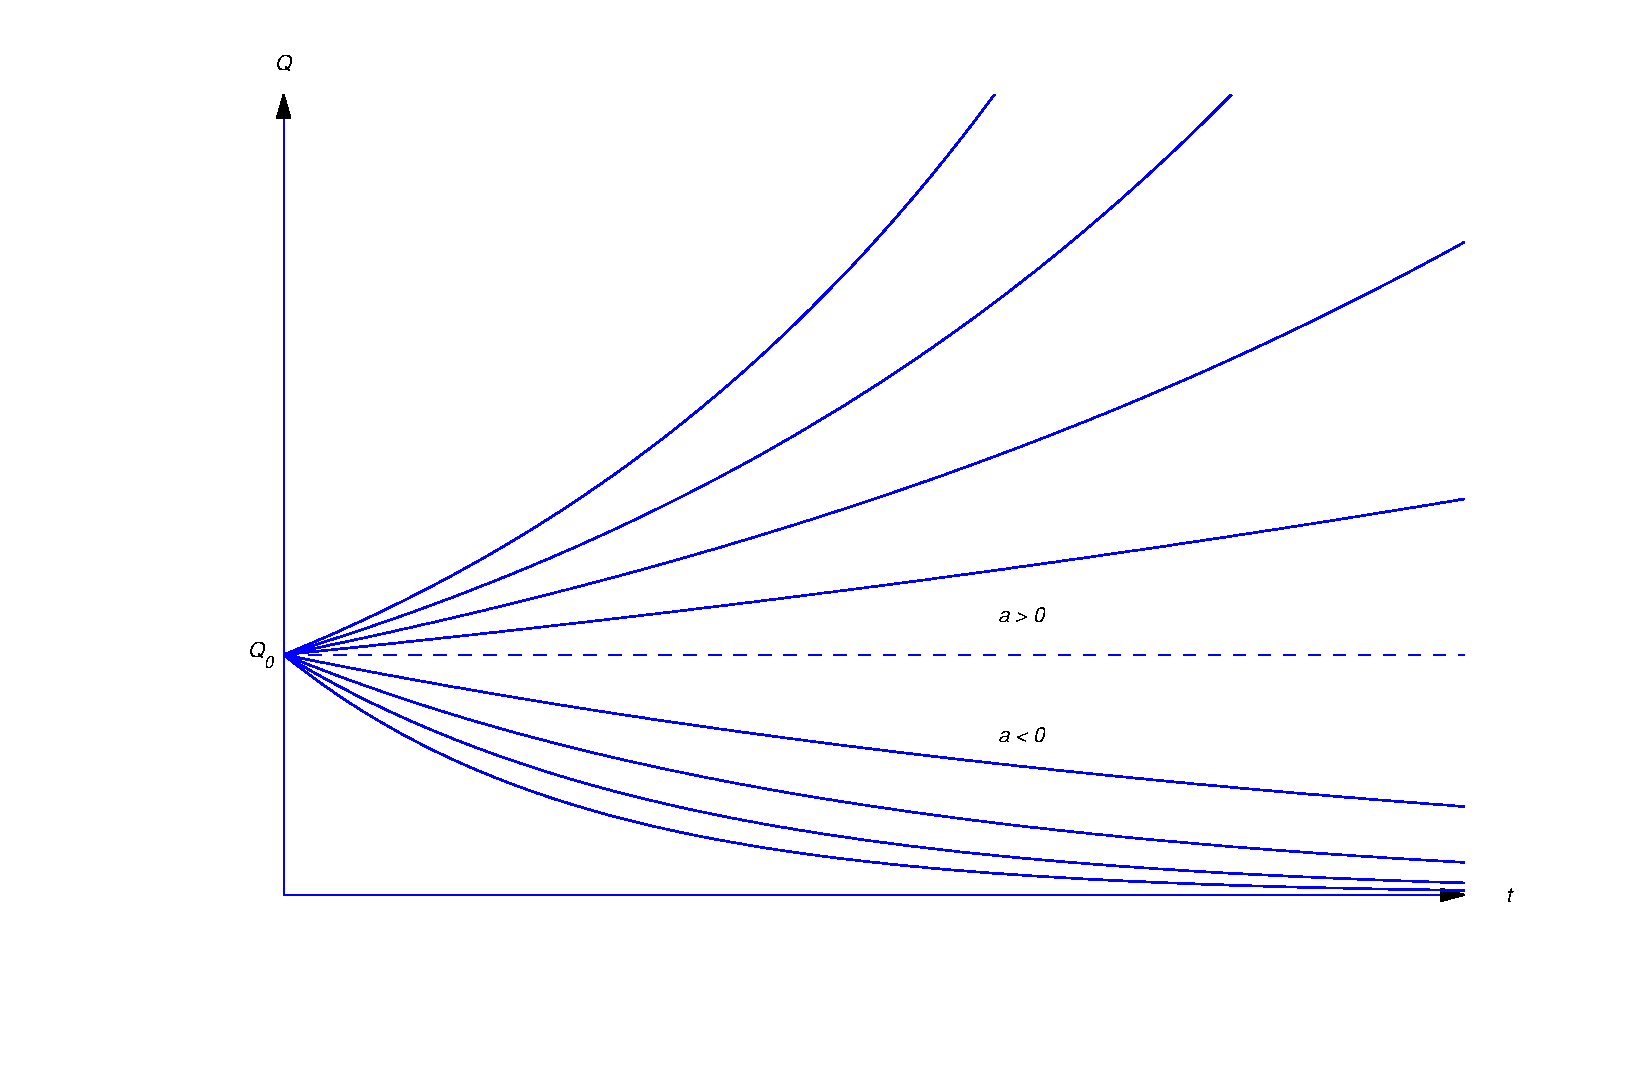
\includegraphics[bb=-78 148 689 643,width=5.67in,height=3.66in,keepaspectratio]{fig040101}
\color{blue}
\caption{\label{figure:4.1.1} Exponential growth  and decay}
  \label{figure4.1.1}
\end{figure}

\boxit{Radioactive Decay}

\noindent
Experimental evidence shows that radioactive material decays at a rate
proportional to the mass of the material present. According to this
model the mass $Q(t)$ of a radioactive material present at time $t$
satisfies \eqref{eq:4.1.1}, where $a$ is a negative constant whose value
for any given material must be determined by experimental observation.
For simplicity, we'll replace the negative constant $a$ by
$-k$, where
$k$ is a positive number that we'll call the {\color{blue}\it decay constant\/}
of the material. Thus, \eqref{eq:4.1.1} becomes
$$
Q'=-kQ.
$$
If the mass of the material present
at $t=t_0$ is $Q_0$,  the mass present at time $t$ is
 the solution of
$$
Q'=-kQ,\quad  Q(t_0)=Q_0.
$$
From \eqref{eq:4.1.2}  with $a=-k$, the solution of this initial value
problem is
\begin{equation} \label{eq:4.1.3}
Q=Q_0e^{-k(t-t_0)}.
\end{equation}

The {\color{blue}\it half--life} $\tau$ of a radioactive material is defined to be
the time required for half of its mass to decay; that is, if
$Q(t_0)=Q_0$, then \begin{equation} \label{eq:4.1.4} Q(\tau+t_0)={Q_0\over
2}.
\end{equation}
 From \eqref{eq:4.1.3} with $t=\tau+t_0$, \eqref{eq:4.1.4} is equivalent to
$$
Q_0e^{-k\tau}={Q_0\over 2},
$$
 so
$$
e^{-k\tau}={1\over 2}.
$$
 Taking logarithms  yields
$$
-k\tau=\ln{1\over 2}=-\ln2,
$$
 so the half-life is
\begin{equation} \label{eq:4.1.5}
\tau={1\over k}\ln2.
\end{equation}
(Figure \ref{figure:4.1.2}). The half-life is independent of $t_0$ and
$Q_0$, since it's determined by the properties of material, not by
the amount of the material present at any particular time.

\begin{figure}[tbp]
  \centering
  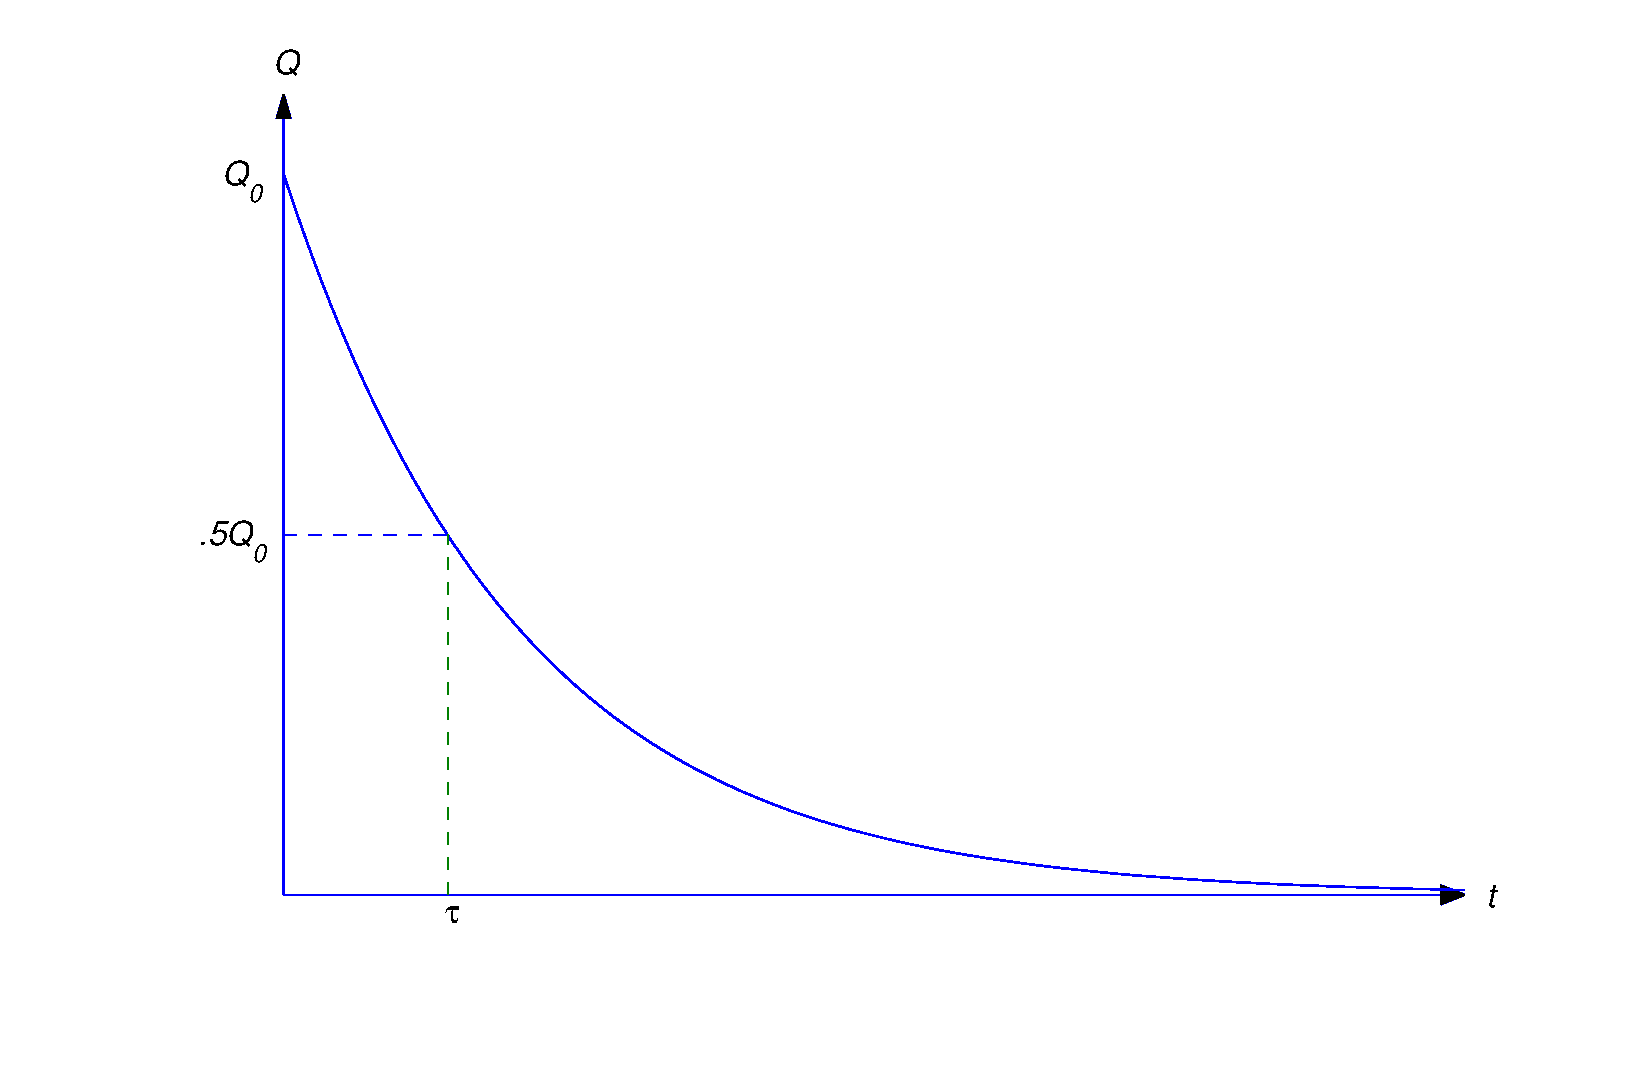
\includegraphics[bb=-78 148 689 643,width=5.67in,height=3.66in,keepaspectratio]{fig040102}
\color{blue}
\caption{Half-life of a radioactive substance}
  \label{figure:4.1.2}
\end{figure}

\begin{example}\label{example:4.1.1} \rm
A  radioactive substance has a half-life of 1620 years.
\begin{alist}
\item %(a)
If its mass is now 4 g (grams), how much will be left 810 years
from now?
\item % (b)
Find the time $t_1$ when 1.5 g of the substance remain.
\end{alist}
\end{example}

\solutionpart{a}  From \eqref{eq:4.1.3} with $t_0=0$ and
$Q_0=4$,
\begin{equation} \label{eq:4.1.6}
Q=4e^{-kt},
\end{equation}
 where we determine $k$ from \eqref{eq:4.1.5}, with $\tau$=
1620 years:
$$
k={\ln2\over\tau}={\ln2\over 1620}.
$$
 Substituting this in \eqref{eq:4.1.6} yields
\begin{equation} \label{eq:4.1.7}
Q=4e^{-(t\ln2)/1620}.
\end{equation}
 Therefore the mass left after 810 years will be
$$\begin{array}{rl}
Q(810) &=4e^{-(810\ln2)/1620}=4e^{-(\ln2)/2} \\
&=2\sqrt{2} \mbox{ g}.
\end{array}$$

\solutionpart{b}
 Setting $t=t_1$  in \eqref{eq:4.1.7} and requiring that
$Q(t_1)=1.5$ yields
$$
{3\over2}=4e^{(-t_1\ln2)/1620}.
$$
Dividing by 4 and taking logarithms yields
$$
\ln{3\over8}=-{t_1\ln2\over1620}.
$$
Since $\ln3/8=-\ln8/3$,
$$
t_1=1620{\ln8/3\over\ln2}\approx  2292.4\;\mbox{ years}.
$$

\boxit{Interest Compounded Continuously}

\noindent
Suppose we deposit an amount of money $Q_0$  in an
interest-bearing account and make no further deposits or withdrawals
for $t$ years, during which the account bears interest at a constant
annual rate $r$. To calculate the value of the account at the
end of $t$ years, we need one more piece of information: how the
interest is added to the account, or---as the bankers say---how it
is {\color{blue}\it compounded}. If the interest is compounded annually,  the
value of the account is multiplied by $1+r$ at the end of each year.
This means that after $t$ years the value of the account is
$$
Q(t)=Q_0(1+r)^t.
$$
If interest is compounded semiannually,  the
value of the account is multiplied by $(1+r/2)$ every 6 months.
Since this occurs twice annually, the value of the account after $t$
years is
$$
Q(t)=Q_0\left(1+{r\over 2}\right)^{2t}.
$$
In general, if interest is compounded $n$ times per year, the value of
the account is multiplied $n$ times per year by $(1+r/n)$;  therefore,
the value of the account
after $t$ years is
\begin{equation} \label{eq:4.1.8}
Q(t)=Q_0\left(1+{r\over n}\right)^{nt}.
\end{equation}
Thus, increasing the  frequency of  compounding increases the value of the
account after a fixed period of time. Table~\ref{table:4.1.1} shows the
effect
of increasing the number of compoundings over $t=5$ years on an initial
deposit of $Q_0=100$ (dollars), at an annual interest rate of 6\%.

\medskip

\begin{newtable} \label{table:4.1.1}
The effect of
compound interest
\begin{center}
$$\begin{array}{|c|c|}\hline
n & \dst\$100 \left(1+{.06\over n}\right)^{5n}\\
\hbox{(number of compoundings} &   \hbox{(value in dollars}\\
\hbox{per year)} &\hbox{after 5 years)}\\
\hline
1 & \$133.82 \\
2 & \$134.39 \\
4 & \$134.68 \\
8 & \$134.83 \\
364 & \$134.98 \\\hline
\end{array}$$
\end{center}
\end{newtable}

\medskip
You can see from Table~\ref{table:4.1.1}  that the value of the account after 5
years is an increasing function of $n$. Now suppose  the maximum
allowable rate of interest on savings accounts is restricted by law,
but the time intervals between successive compoundings isn't ; then
competing banks can attract savers by compounding often. The ultimate
step in this direction is to {\color{blue}\it compound continuously}, by which we
mean that $n\to\infty$ in \eqref{eq:4.1.8}. Since we know from calculus
that
$$
\lim_{n\to\infty} \left(1+{r\over n}\right)^n=e^r,
$$
 this yields
$$\begin{array}{rl}
Q(t) & \dst=\lim_{n\to\infty} Q_0\left(1+{r\over
n}\right)^{nt}=Q_0 \left[
\lim_{n\to\infty} \left(1+{r\over n}\right)^n\right]^t \\[12pt]
&=Q_0e^{rt}.
\end{array}$$
Observe that $Q=Q_0e^{rt}$ is the solution of the initial value problem
$$
Q'=rQ, \quad Q(0)=Q_0;
$$
 that is, with continuous compounding the value of the account
grows exponentially.

\begin{example}\label{example:4.1.2} \rm
If \$150 is deposited in a bank that pays
$5{1\over2}$\% annual
interest compounded continuously,  the value of the account after
$t$ years is
$$
Q(t)=150e^{.055t}
$$
dollars. (Note that it's necessary to write the interest rate as a
decimal;   thus, $r=.055$.) Therefore, after $t=10$ years the value
of the account is
$$
Q(10)=150e^{.55} \approx \$259.99.
$$
\end{example}

\begin{example}\label{example:4.1.3} \rm
We wish to accumulate \$10,000 in 10 years by making a single deposit
in a savings account bearing $5{1\over2}$\% annual interest
compounded continuously. How much must we deposit in the account?
\end{example}

\solution  The value of the account at time $t$ is
\begin{equation} \label{eq:4.1.9}
Q(t)=Q_0e^{.055t}.
\end{equation}
Since we want $Q(10)$ to be \$10,000, the initial deposit $Q_0$ must
satisfy the equation
\begin{equation} \label{eq:4.1.10}
10000=Q_0e^{.55},
\end{equation}
 obtained by setting $t=10$ and $Q(10)=10000$ in
\eqref{eq:4.1.9}.  Solving \eqref{eq:4.1.10} for $Q_0$ yields
$$
Q_0=10000e^{-.55} \approx \$5769.50.
$$

\boxit{Mixed Growth and Decay}

\begin{example}\label{example:4.1.4} \rm
A radioactive substance with decay constant $k$ is produced at a
constant rate of $a$ units of mass per unit time.
\begin{alist}
\item %(a)
Assuming that $Q(0)=Q_0$, find the mass $Q(t)$ of the
substance present at time~$t$.

\item %(b)
Find $\lim_{t\to\infty} Q(t)$.
\end{alist}
\end{example}

\solutionpart{a}  Here
$$
Q'=\mbox{ rate of increase of } Q - \mbox{ rate of decrease
of } Q.
$$
The rate of increase is the constant $a$. Since $Q$ is radioactive
with decay constant $k$, the rate of decrease is $kQ$. Therefore
$$
Q'=a-kQ.
$$
This is a linear first order differential equation. Rewriting it and
imposing the initial condition shows that $Q$ is the solution of the
initial value problem
\begin{equation}  \label{eq:4.1.11}
Q'+kQ=a, \quad Q(0)=Q_0.
\end{equation}
Since
$e^{-kt}$ is a solution of the complementary equation, the solutions
of \eqref{eq:4.1.11} are of the form $Q=ue^{-kt}$, where $u'e^{-kt}=a$, so
$u'=ae^{kt}$. Hence,
$$
u={a\over k}e^{kt}+c
$$
and
$$
Q=ue^{-kt}={a\over k}+ce^{-kt}.
$$
 Since $Q(0)=Q_0$, setting $t=0$ here yields
$$
Q_0={a\over k}+c  \mbox{\quad or \quad} c=Q_0-{a\over k}.
$$
 Therefore
\begin{equation} \label{eq:4.1.12}
Q={a\over k}+\left(Q_0-{a\over k}\right)e^{-kt}.
\end{equation}

\solutionpart{b}
Since $k > 0$,  $\lim_{t\to\infty} e^{-kt}=0$, so
from \eqref{eq:4.1.12}
$$
\lim_{t\to\infty} Q(t)={a\over k}.
$$
This limit depends only on $a$ and $k$, and not on $Q_0$.
We say that $a/k$ is the {\color{blue}\it steady state} value of $Q$. From
\eqref{eq:4.1.12} we also see that $Q$ approaches its steady state value
from above if $Q_0 > a/k$, or from below if $Q_0 < a/k$. If $Q_0=a/k$,
then $Q$ remains constant (Figure \ref{figure:4.1.3}).

\begin{figure}[tbp]
  \centering
  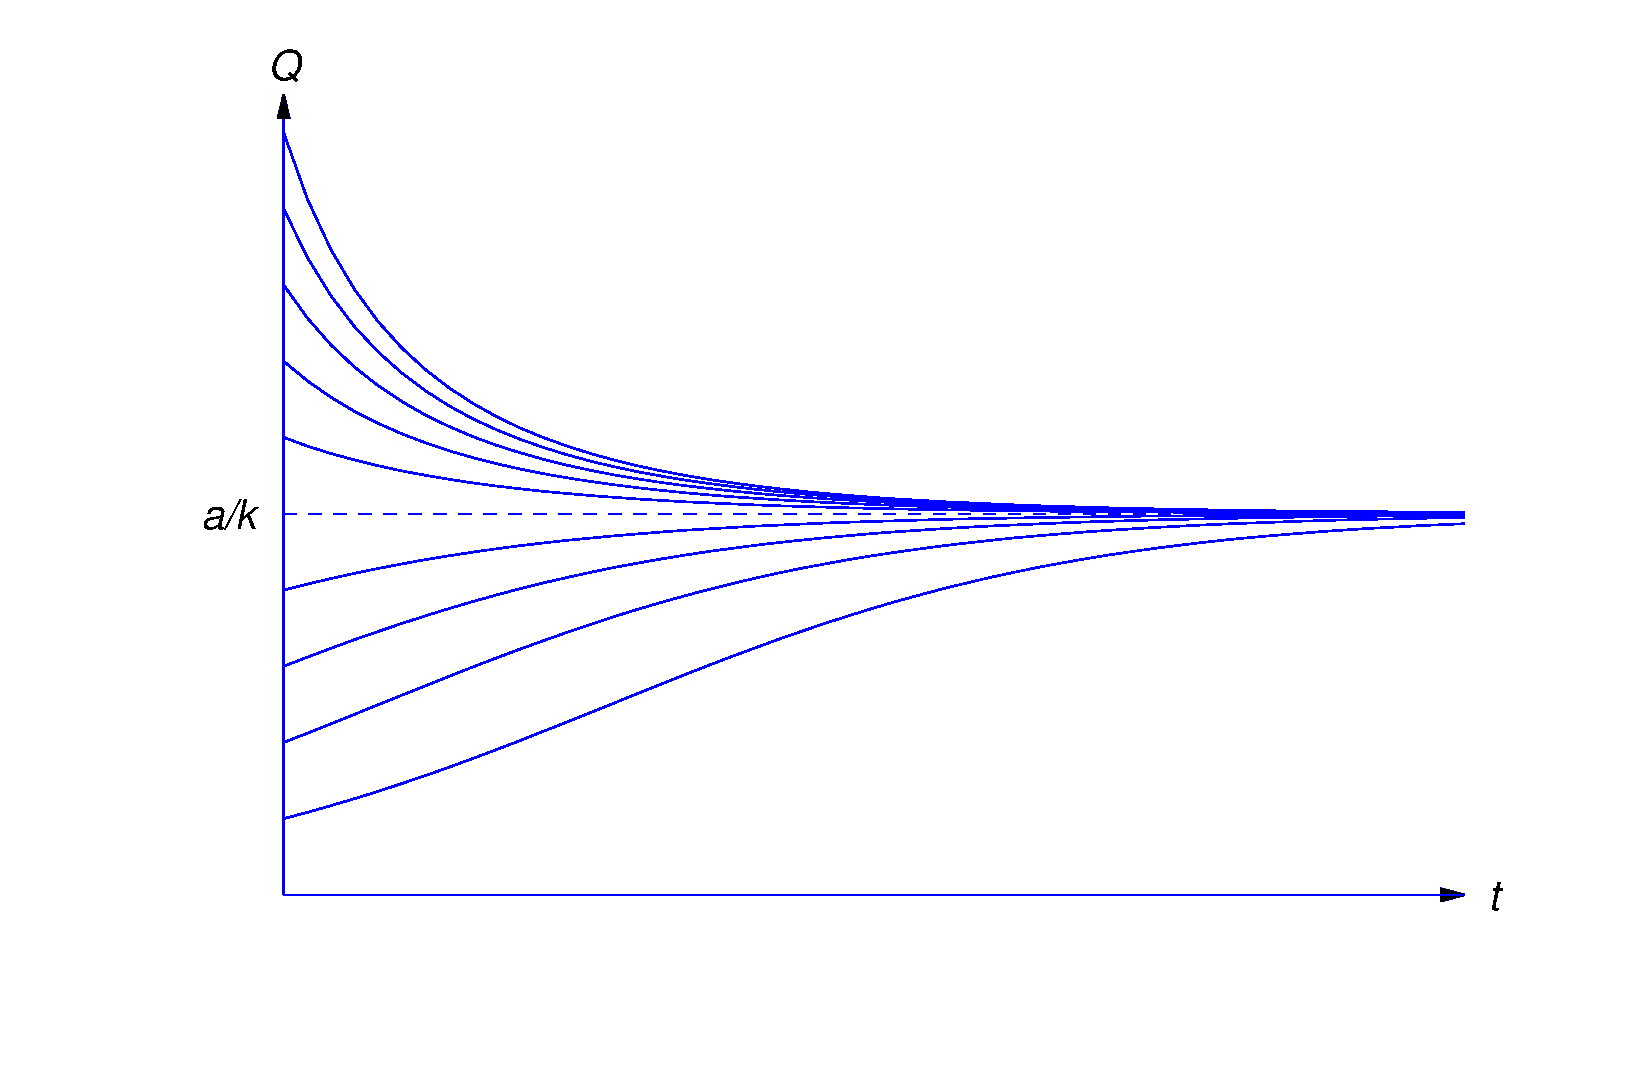
\includegraphics[bb=-78 148 689 643,width=5.67in,height=3.66in,keepaspectratio]{fig040103}
\color{blue}
\caption{$Q(t)$ approaches the steady state value
$\dst{a\over k}$ as $t\to\infty$}
  \label{figure:4.1.3}
\end{figure}

\boxit{Carbon Dating}

\noindent
The fact that $Q$ approaches a steady state value in the
situation discussed in Example 4 underlies the method of {\color{blue}\it carbon
dating}, devised by  the American chemist  and Nobel Prize Winner
\href{https://www.nobelprize.org/uploads/2018/06/libby-lecture.pdf}
{\color{blue}\it W.S. Libby}.

Carbon 12 is stable, but carbon-14, which is produced by cosmic
bombardment of nitrogen in the upper atmosphere, is radioactive with a
half-life of about 5570 years. Libby assumed that the
quantity
of carbon-12 in the atmosphere has been constant throughout time, and
that the quantity of radioactive carbon-14 achieved its steady state
value long ago as a result of its creation and decomposition over
millions of years. These assumptions led Libby to conclude that the
ratio of carbon-14 to carbon-12 has been nearly constant for a long
time. This constant, which we denote by $R$, has been determined
experimentally.

Living cells absorb both carbon-12 and carbon-14 in the proportion in
which they are present in the environment. Therefore the ratio of
carbon-14 to carbon-12 in a living cell is always $R$. However, when
the cell dies it ceases to absorb carbon, and the ratio of carbon-14
to carbon-12 decreases exponentially as the radioactive carbon-14
decays. This is the basis for the method of carbon dating, as
illustrated in the next example.

\begin{example}\label{example:4.1.5} \rm
An archaeologist investigating the site of an ancient village finds a
burial ground where the amount of carbon-14 present in individual
remains is between 42 and 44\% of the amount present in live
individuals. Estimate the age of the village and the length of time
for which it survived.
\end{example}

\solution Let $Q=Q(t)$ be the quantity of carbon-14 in an individual
set of remains $t$ years after death, and let $Q_0$ be the quantity
that would be present in  live individuals.
Since carbon-14 decays exponentially with half-life 5570 years, its
decay constant is
$$
k={\ln2\over 5570}.
$$
 Therefore
$$
Q=Q_0e^{-t(\ln2)/5570}
$$
 if we choose our time scale so that $t_0=0$ is the
time of death.  If we know the present value of $Q$  we
can solve this equation for $t$, the number of years since
death occurred.  This yields
$$
t=-5570 {\ln Q/Q_0\over\ln2}.
$$
It is given that $Q=.42Q_0$ in the remains of individuals who died
first. Therefore these deaths occurred about
$$
t_1=-5570 {\ln .42\over\ln2} \approx 6971
$$
 years ago.  For the most recent deaths, $Q=.44
Q_0$; hence, these deaths occurred about
$$
t_2=-5570 {\ln .44\over\ln2} \approx 6597
$$
 years ago.  Therefore it's reasonable to conclude
that the village was founded about 7000 years ago,
and lasted for about 400 years.

\boxit{A Savings Program}

\vspace*{-.2in}
\noindent
\begin{example}\label{example:4.1.6} \rm
A person opens a savings account with an initial deposit of \$1000 and
subsequently deposits \$50 per week. Find the value $Q(t)$ of the
account at time $t > 0$, assuming that the bank pays 6\%
interest compounded continuously.
\end{example}

\solution Observe that $Q$ isn't  continuous, since there are 52
discrete deposits per year of \$50 each. To construct a mathematical
model for this problem in the form of a differential equation, we make
the simplifying assumption that the deposits are made continuously at
a rate of \$2600 per year. This is essential, since solutions of
differential equations are continuous functions. With this assumption,
$Q$ increases continuously at the rate
$$
Q'=2600+.06 Q
$$
and therefore $Q$ satisfies the differential equation
\begin{equation} \label{eq:4.1.13}
Q'-.06Q=2600.
\end{equation}
(Of course, we must recognize that the solution of this equation
is an approximation to the true value of $Q$ at any given time. We'll
discuss this further below.)  Since $e^{.06t}$ is a solution of the
complementary equation, the solutions of \eqref{eq:4.1.13}  are of the
form   $Q=ue^{.06t}$,  where $u'e^{.06t}=2600$. Hence,
$u'=2600e^{-.06t}$,
$$
u=- {2600\over .06}e^{-.06t}+c
$$
and
\begin{equation} \label{eq:4.1.14}
Q=ue^{.06t}=-{2600\over .06}+ce^{.06t}.
\end{equation}
 Setting $t=0$ and $Q=1000$ here yields
$$
c=1000+{2600\over .06},
$$
and substituting this into \eqref{eq:4.1.14} yields
\begin{equation} \label{eq:4.1.15}
Q=1000e^{.06t}+{2600\over .06}(e^{.06t}-1),%\tag15
\end{equation}
where the first term is the value due to the initial deposit and the
second is due to the subsequent weekly deposits. \bbox

Mathematical models must be tested for validity by comparing
predictions based on them with the actual outcome of experiments.
Example 6 is unusual in that we can compute the exact value of the
account at any specified time and compare it with the approximate
value predicted by \eqref{eq:4.1.15} (See Exercise \ref{exer:4.1.21}.). The
follwing table
 gives a comparison for a ten year period. Each exact answer
corresponds to the time of the year-end deposit, and each year is
assumed to have exactly 52 weeks.

$$
\vbox{\tabskip=0pt \offinterlineskip
\def\tablerule{\noalign{\hrule}}
\halign{\hfill#\hfill&\qquad\hfill#\hfill&\qquad\hfill#\hfill
  &\qquad\hfill#\hfill&\qquad#\hfill\cr
%\noalign{\centerline{\bf Table \label{table:4.1.2}}}
\noalign{\vskip12pt}
%\noalign{\centerline{Value of the Saver's Account (Example
%\ref{example:4.1.6})}}
\noalign{\vskip22pt}
Year & Approximate Value of $Q$ & Exact Value of  $P$ & Error & Percentage
Error
\cr & (Example~\ref{example:4.1.6}) & (Exercise~\ref{exer:4.1.21}) & $Q-P$ &\ \;
$(Q-P)/P$ \cr \noalign{\vskip16pt}
\  1 & \$ 3741.42 & \$ 3739.87 & \$ 1.55 &\ \; $.0413 $\% \cr
\noalign{\vskip7pt}
\  2 &\  \, 6652.36 &\ \;  6649.17 &\ \; 3.19 &\ \; $.0479$
\cr
\noalign{\vskip7pt}
\  3 &\  \, 9743.30 &\ \;  9738.37 &\ \; 4.93 &\ \; $.0506$
\cr
\noalign{\vskip7pt}
\  4 & \, 13,025.38 & \, 13,018.60 &\ \; 6.78 &\ \; $.0521$
\cr
\noalign{\vskip7pt}
\  5 & \, 16,510.41 & \, 16,501.66 &\ \; 8.75 &\ \; $.0530 $
\cr
\noalign{\vskip7pt}
\  6 & \, 20,210.94 & \, 20,200.11 & 10.83 &\ \; $.0536$
\cr
\noalign{\vskip7pt}
\  7 & \, 24,140.30 & \, 24,127.25 & 13.05 &\ \; $.0541 $
\cr
\noalign{\vskip7pt}
\  8 & \, 28,312.63 & \, 28,297.23 & 15.40 &\ \; $.0544 $
\cr
\noalign{\vskip7pt}
\  9 & \, 32,742.97 & \, 32,725.07 & 17.90 &\ \; $.0547 $
\cr
\noalign{\vskip7pt}
10 & \, 37,447.27 & \, 37,426.72 & 20.55 &\ \; $.0549 $ \cr}}
$$
\newpage

\exercises

\begin{exerciselist}
\item\label{exer:4.1.1}
The half-life of a radioactive substance is 3200
years.  Find the quantity $Q(t)$ of the substance left at
time $t > 0$ if $Q(0)=20$ g.

\item\label{exer:4.1.2}
The half-life of a radioactive substance is 2 days.  Find
the time required for a given amount of the material to
decay to 1/10 of its original mass.

\item\label{exer:4.1.3}
A  radioactive material loses 25\% of its mass
in 10 minutes.  What is its half-life?

\item\label{exer:4.1.4}
A  tree contains a known percentage $p_0$ of
a radioactive substance with half-life $\tau$.  When the
tree dies the substance decays and isn't  replaced.  If the
percentage of the substance in the fossilized remains of
such a tree is found to be $p_1$, how long has the tree been
dead?

\item\label{exer:4.1.5}
If $t_p$ and $t_q$ are the times required for a radioactive
material to decay to $1/p$ and $1/q$  times
its original mass (respectively), how are $t_p$ and $t_q$ related?

\item\label{exer:4.1.6}
Find the decay constant $k$ for a radioactive substance,
given that the mass of the substance is $Q_1$ at time $t_1$
and $Q_2$ at time $t_2$.

\item\label{exer:4.1.7}
A process creates a radioactive substance at the rate of 2
g/hr and the substance decays at a rate proportional to
its mass, with constant of proportionality
$k=.1 (\mbox{hr})^{-1}$.  If $Q(t)$ is the mass of the
substance at time $t$, find $\lim_{t\to\infty}Q(t)$.

\item\label{exer:4.1.8}
A bank pays interest continuously at the rate of 6\%.
How long does it take for a deposit of $Q_0$ to grow in
value to $2Q_0$?

\item\label{exer:4.1.9}
At what rate of interest, compounded continuously, will a
bank deposit double in value in 8 years?

\item\label{exer:4.1.10}
A savings account pays 5\% per annum interest compounded
continuously. The initial deposit is $Q_0$ dollars. Assume that there
are no subsequent withdrawals or deposits.
\begin{alist}
\item % (a)
How long will it take for the value of the account to triple?
\item % (b)
What is $Q_0$ if the value of the account after 10 years is \$100,000
dollars?
\end{alist}

\item\label{exer:4.1.11}
A candymaker makes 500 pounds of candy per week, while
his large family eats the candy at a rate equal to $Q(t)/10$
pounds per week, where $Q(t)$ is the amount of candy present
at time $t$.
\begin{alist}
\item %(a)
Find $Q(t)$ for $t > 0$ if the candymaker has 250 pounds of
candy at $t=0$.
\item %(b)
Find $\lim_{t\to\infty} Q(t)$.
\end{alist}

\item\label{exer:4.1.12}
Suppose a substance decays at a yearly rate  equal
to half the square of the mass of the substance present.  If
we start with 50 g of the substance, how long will it be
until only 25 g remain?

\item\label{exer:4.1.13}
A super bread dough increases in volume at a rate
proportional to the volume $V$ present.  If $V$ increases by
a factor of 10 in 2 hours and $V(0)=V_0$, find $V$ at any
time $t$.  How long will it take for $V$ to increase to $100
V_0$?

\item\label{exer:4.1.14}
A radioactive substance decays at a rate proportional to the
amount present, and half the original quantity $Q_0$ is left
after 1500 years. In how many years would the original
amount be reduced to $3Q_0/4$?  How much will be
left after 2000 years?

\item\label{exer:4.1.15}
A wizard creates gold continuously at the rate of 1 ounce
per hour, but an assistant steals it continuously at the
rate of 5\% of however much  is there per hour.  Let $W(t)$
be the number of ounces that the wizard has at time $t$.
Find $W(t)$ and $\lim_{t\to\infty}W(t)$ if  $W(0)=1$.

\item\label{exer:4.1.16}
A process creates a radioactive substance at the rate of 1
g/hr, and the substance decays at an hourly rate
 equal to 1/10 of the mass present (expressed in
grams).  Assuming that there are initially 20 g, find
the mass $S(t)$ of the substance present at time $t$, and
find $\lim_{t\to\infty} S(t)$.

\item\label{exer:4.1.17}
A tank is empty at $t=0$.  Water is added to the tank at
the rate of 10 gal/min, but it leaks out at a rate
 (in gallons per minute)  equal to the number of
gallons in the tank.  What is the smallest capacity the tank
can have if this process is to continue forever?

\item\label{exer:4.1.18}
A person deposits \$25,000 in a bank that pays 5\% per
year interest, compounded continuously.  The person
continuously withdraws from the account at the rate of \$750
per year.  Find $V(t)$, the value of the account at time $t$
after the initial deposit.

\item\label{exer:4.1.19}
  A person has a fortune that grows at rate proportional to the
square root of its worth. Find the  worth $W$ of the fortune as a function
of $t$ if it was  \$1 million 6 months ago and
is \$4 million today.

\item\label{exer:4.1.20}
Let $p=p(t)$ be the quantity of a  product present at
time $t$. The product is manufactured continuously at a
rate proportional to $p$, with proportionality constant 1/2,
and it's consumed continuously at a rate proportional to
$p^2$, with proportionality constant 1/8.  Find $p(t)$ if
$p(0)=100$.

\item\label{exer:4.1.21}

\begin{alist}
\item % (a)
 In the situation of Example~\ref{example:4.1.6}
find the exact value $P(t)$ of the person's account after $t$
years, where $t$ is an integer.  Assume that each year has
exactly 52 weeks, and include the year-end
deposit in the computation.

\hint{At time $t$ the initial $\$1000$
has been on deposit for $t$ years.  There have been $52t$
deposits of $\$50$ each.  The first $\$50$ has been on deposit
for $t-1/52$ years, the second for $t-2/52$ years $\cdots$
in general, the $j$th $\$50$ has been on deposit for $t-j/52$
years $(1 \le j \le 52t)$.  Find the present value of each
$\$50$ deposit assuming $6$\% interest compounded
continuously, and use the formula
$$
1+x+x^2+\cdots+x^n={1-x^{n+1}\over 1-x}\
(x \ne 1)
$$
to find their total value.}

\item % (b)
 Let
$$
p(t)={Q(t)-P(t)\over P(t)}
$$
be the relative error after $t$ years.  Find
$$
p(\infty)=\lim_{t\to\infty}p(t).
$$
\end{alist}

\item\label{exer:4.1.22}
A homebuyer borrows $P_0$ dollars at an annual interest rate $r$,
agreeing to repay the loan with equal monthly payments of $M$ dollars
per month over $N$ years.
\begin{alist} \item % (a)
Derive a
differential equation for the loan principal (amount that the
homebuyer owes) $P(t)$ at time $t>0$, making the simplifying
assumption that the homebuyer repays the loan continuously rather than
in discrete steps. (See Example~\ref{example:4.1.6} .)

\item %(b)
Solve the equation derived in \part{a}.

\item % (c)
 Use the result of \part{b} to determine an approximate
value for $M$  assuming that each year has exactly 12 months of
equal length.

\item % (d)
 It can be shown that the exact value of $M$  is given by
$$
M={rP_0\over 12}\left(1-(1+r/12)^{-12N}\right)^{-1}.
$$
Compare    the value of $M$ obtained from the answer in \part{c} to the
exact value  if
 (i) $P_0=\$50,000$, $r=7{1\over2}$\%, $N=20$
 (ii) $P_0=\$150,000$, $r=9.0$\%, $N=30$.
\end{alist}

\item\label{exer:4.1.23}
Assume that the homebuyer of Exercise \ref{exer:4.1.22} elects to repay the
loan continuously at the rate of $\alpha M$ dollars per month,
where $\alpha$ is a constant greater than 1. (This is called {\color{blue}\it
accelerated payment\/}.)
\begin{alist}
\item % (a)
 Determine the time $T(\alpha)$ when the loan
will be paid off and the amount $S(\alpha)$ that the homebuyer will save.

\item % (b)
 Suppose $P_0=\$50,000$, $r=8$\%, and $N=15$.
Compute
the savings realized by accelerated payments with $\alpha=1.05,1.10$, and
$1.15$.
\end{alist}

\item\label{exer:4.1.24} A benefactor wishes to establish a trust fund to
pay a researcher's salary for $T$ years. The salary is to start at
$S_0$ dollars per year and increase at a fractional rate of $a$ per
year. Find the amount of money $P_0$ that the benefactor must deposit
in a trust fund paying interest at a rate $r$ per year. Assume that
the researcher's salary is paid continuously, the interest is
compounded continuously, and the salary increases are granted
continuously.

\item\label{exer:4.1.25} \Lex
A radioactive substance with decay constant $k$ is produced
at the rate of
$$
{at\over1+btQ(t)}
$$
 units of mass per unit time, where
$a$ and $b$ are positive constants and $Q(t)$ is the mass of the
substance present at time $t$;   thus, the rate of production is small
at the start
 and tends to slow when $Q$ is large.
\begin{alist}
\item % (a)
Set up a differential equation for $Q$.
\item % (b)
Choose your own positive values for $a$, $b$, $k$, and
$Q_0=Q(0)$.
Use a numerical method
to discover what happens to $Q(t)$
as $t\to\infty$. (Be precise, expressing your conclusions in terms of
$a$, $b$, $k$. However,  no proof is required.)
\end{alist}

\item\label{exer:4.1.26} \Lex
Follow the instructions of Exercise~\ref{exer:4.1.25}, assuming that
the substance is produced at the rate of   $at/(1+bt(Q(t))^2)$
units of mass per unit of time.

\item\label{exer:4.1.27} \Lex
Follow the instructions of Exercise~\ref{exer:4.1.25}, assuming that
the substance is produced at the rate of   $at/(1+bt)$
units of mass per unit of time.

\end{exerciselist}
